\section{Begriffe und Elemente}\label{sec:klassendiagramme-begriffe-und-elemente}

\subsection{Properties}
Es gibt zwei unterschiedliche Notationen für Properties: Die \textbf{Attribut}- und die \textbf{Assoziationsnotation}.

\subsubsection*{Attributnotation}

\begin{itemize}
    \item \textbf{Attributnotation}: Textzeile innerhalb des zweiten \textit{Compartments} der Klassenbox.\\
    Neben \textbf{Instanzattributen}, die die Eigenschaften eines Objektes charakterisieren, können auch \textbf{Klassenattribute} angegeben werden: Der Bezeichner wird dann \underline{unterstrichen}.\\
    Die formale Notation für ein Attribut lautet:\\
    \medskip
     \noindent
    \begin{small}
        \textcolor{blue}{[Sichtbarkeit][/] name [:Typ][[Multiplizität]][=Vorgabewert][\{Eigenschaftswert [, Eigenschaftswert]*\}]}\\
    \end{small}
    \noindent
    Eckige Klammern stehen hierbei für \textit{optionale} Angaben\footnote{
        die \textbf{Multipliziät} wird immer in eckigen Klammern angegeben, das zweite Klammernpaar steht hier für die optionale Angabe
    }.
    \begin{itemize}
        \item \textbf{Sichtbarkeit}:
            \begin{itemize}
                \item \code{+} \textit{public}
                \item \code{#} \textit{protected}
                \item \code{-} \textit{private}
                \item \code{~} \textit{package private}
            \end{itemize}
        \item \textbf{/}: es handelt sich um ein \textbf{abgeleitetes Attribut}\footnote{
            \textit{abgeleitet}: der Wert wird berechnet und nicht durch den Anwender angegeben oder aus einer externen Quelle geladen
        }. Bei abgeleiteten Attributen ist zu prüfen, ob sie  die Attribute zu speichern oder jeweils aktuell zu berechnen ``und daher in Operationen zu wandeln sind`` (\cite[414]{Bal05}). Eine Zwischenspeicherung als Attribut ist bspw. dann sinnvoll, wenn die Berechnung komplex und kostenintensiv ist.
        \item \textbf{Multiplizität}:
        \begin{itemize}
            \item \code{[0..*]}: optionales Attribut, gekennzeichnet durch $0$ als untere Grenze.
            Der Stern \code{*} zeigt an, dass bel. viele Ausprägungen vorhanden sein dürfen.
            Statt \code{[0..*]} kann in dem Fall auch \code{[*]} notiert werden.
            \item \code{[1..n]}: obligatorische Property, gekennzeichnet durch $1$ als untere Grenze ($1 \leq n < \infty, n \in \mathbb{N}$):
            \item \code{[1]}: Standardwert
        \end{itemize}
        \item \textbf{Vorgabewert}: Initialisierungswert
        \item \textbf{Eigenschaftswert}: \textit{Tagged Values}.
        Stellen besondere Eigenschaftswerte bezogen auf das \textbf{Modellelement} (hier: \textit{Attribut}) dar, {bspw.} \code{{readOnly}}, \code{{ordered}}, \code{{frozen}} usw. Werden keine Vorgaben der UML genutzt, hat der Eigenschaftswert die Form \code{{Eigenschaft=Wert}} (so ist bspw. \code{{readOnly}} eine Kurzschreibweise für  \code{{readOnly=true}})
        \item \textbf{Einschränkungen}: Zusätzliche Einschränkungen, bspw. in der Notation der \textbf{OCL}, werden ebenfalls in geschweiften Klammern angegeben.\\
        Man spricht in diesem Zusammenhang auch von \textbf{(Klassen-)Invarianten}: Eigenschaften von Attributen, die für jedes Objekt der Klasse gelten (vgl.\cite[338]{Oes05}).
        Diese Anforderungen, die das Attribut erfüllen muss, müssen als boolescher Ausdruck formuliert werden, so dass die Anforderung zu \code{true} oder \code{false} ausgewertet werden kann.
        Einschränkungen können direkt hinter das Attribut, als Notiz oder ausgelagert in einer Textdatei angegeben werden.
    \end{itemize}

\end{itemize}

\vspace{2mm}
\begin{tcolorbox}[title=Fehlende Angaben zur Multiplizität]
    \textit{Fowler} empfiehlt die Angabe von \textbf{Multiplizitäten}, um Unklarheiten zu vermeiden: Wird eine Multiplizität nicht angegeben, kann der Autor damit ausdrücken wollen, dass die Standard-Multiplizität $[1]$ gemeint ist - es kann aber auch sein, dass einfach keine Angaben dazu im Diagramm gemacht worden sind, weshalb man per se nicht von einer Multiplizität von $[1]$ ausgehen darf.
    \blockquote[{\cite[39]{Fow03b}}]{
        The default implicity of an attribute is [1]. Although this is true in the meta-model, you can't assume that an attribute in a diagram that's missing a multiplicity has a value of [1], as the diagram may be suppressing the multiplicity information. As a result, I prefer to explicitly state a [1] multiplicity if it's important.
    }
\end{tcolorbox}
\vspace{2mm}

\begin{tcolorbox}[title=Nur ein Wert $n > 1$ bei der Multiplizität,colback=red!20]
    In~\cite[19]{Buh09} vermerkt \textit{Buhl}:
    \blockquote{
    [1] - untere Grenze 1 und obere Grenze 1.[\ldots] Ist nur ein Wert angegeben, so wird die untere Grenze grundsätzlich mit 1 angenommen.
    }\\

    \noindent
    Im Gegensatz hierzu findet sich bei \textit{Oestereich}:\\
    \blockquote[{\cite[274, Hervorhebung eigene]{Oes05}}]{
        $0..3,\quad 7,\quad 9..*\quad$ von null bis drei oder \textbf{genau sieben} oder größer oder gleich neun
    }\\
    sowie in der Spezifikation:\\
    \blockquote[{\cite[35]{OMG17}}]{
        If the lower bound is equal to the upper bound, then an alternate notation is to use a string containing just the upper
        bound.
    }\\
    \textit{Balzert} argumentiert in \cite[43]{Bal05} gleich.
\end{tcolorbox}

\subsubsection*{Assoziationsnotation}

\begin{tcolorbox}
    Eine Assoziation repräsentiert die semantische Beziehung zwischen Klassen.
\end{tcolorbox}

\noindent
Die \textbf{Assoziationsnotation} verwendet durchgehende Linien zwischen Klassen.\\

\noindent
Assoziationen können Namen besitzen, die mit einer Leserichtung ausgestattet sind (bspw. durch eine Pfeilspitze).\\

\noindent
\textbf{Assoziationsenden} können darüberhinaus mit folgenden Informationen versehen werden:

\begin{itemize}
    \item \textbf{Rollennamen}, zusätzlich mit \textit{Sichtbarkeiten}
    \item \textbf{Eigenschaftswerte}\footnote{
    ``Die bedeutung der von der UML vorgegebenen Eigenschaftswerte hat gegenüber den Attributen eine leicht abweichende Semantik.`` (\cite[20]{Buh09})
    }
    \item \textbf{Einschränkungen}
    \item \textbf{Multiplizitäten}
\end{itemize}

\noindent
\textbf{Pfeilspitzen} an Assoziationsenden geben die \textbf{Navigierbarkeit} an (s. Abbildung~\ref{fig:navigability}):

\begin{itemize}
    \item \textbf{Bidirektional}: Pfeilspitzen an beiden Enden
    \item \textopf{Unidirektional}: Pfeilspitze an nur einem Ende (\textit{navigabilityNotation}).
    Ein offenes ``X`` (\textit{nonNavigabilityNotation}) an einem Ende weist darauf hin, dass der Zugriff auf diese Seite der Assoziation ausgeschlossen ist (vgl.~\cite[719]{OMG17}).
    \item \textbf{keine Angabe}: bidirektionale Assoziation, oder Navigierbarkeit wurde noch nicht modelliert\footnote{
     zur Vermeidung von Unklarheiten empfiehlt es sich, die Navigierbarkeit anzugeben. S. auch die obige Anmerkung zur \textit{Multiplizität}
    }
\end{itemize}

\begin{figure}
    \centering
    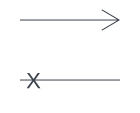
\includegraphics[scale=0.5]{part three/Klassendiagramme/img/navigability}
    \caption{Notation für ein \textit{navigabilityNotation} (oben) und eine \textit{nonNavigabilityNotation} (unten): Die \textit{navigabilityNotation} wird verwendet, wenn ``Indicates when to show navigability of associations or connectors typed by associations``; die \textit{nonNavigabilityNotation}, falls ``Indicates when to show non-navigability of associations or connectors typed by associations.`` (\cite[731]{OMG17}). (Quelle: in Anlehnung an \cite[719]{OMG17})}
    \label{fig:navigability}
\end{figure}

\begin{tcolorbox}[title=Angabe der Navigierbarkeit,colback=white]
    Die UML Spezifikation weist in~\cite[203]{OMG17} darauf hin, dass es möglich ist, durch die gleichzeitige Angabe der \textit{nonNavigabilityNotation} / \textit{navigabilityNotation} die Navigierbarkeit \textit{explizit} darzustellen.\\
    In der Praxis wird häufig nur der Pfeil in eine Richtung verwendet (unidirektionale Assoziation), auf die \textit{nonNavigabilityNotation} wird hingegen verzichtet: In diesem Fall können wir \textit{Balzert} folgen, der die Navigierbarkeit in die andere Richtung als \textit{undefiniert} behandelt (vgl.~\cite[285]{Bal05}).
\end{tcolorbox}

\subsection*{Anmerkungen}
\textit{Buhl} weist darauf hin, dass

\begin{itemize}
    \item Eigenschaftswerte von Properties in einer Implementierung (Java) umgesetzt werden müssen
    \item es günstig ist, Klassen \textit{restriktiv} zu entwerfen: Rechte können in Unterklassen erweitert werden.\\
    Rechte können aber nicht in Unterklassen eingeschränkt werden.
\end{itemize}

\begin{tcolorbox}[title=Attribut- vs. Assoziationsnotation,colback=white]
    Jedes Attribute kann laut UML alternativ zur Textnotation mithilfe von Assoziationen dargestellt werden (vgl.~\cite[264]{Bal05}).\\
    Eine äquivalente Darstellung von einer Attribut- / Assoziationsnotation findet sich in Abbildung~\ref{fig:attassocequiv}.
\end{tcolorbox}


\begin{figure}
    \centering
    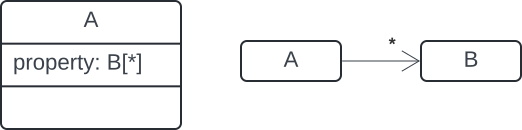
\includegraphics[scale=0.5]{part three/Klassendiagramme/img/attassocequiv}
    \caption{Darstellung eines Attributs in Attribut-/Assoziationsnotation. Die Darstellung sind äquivalent zueinander. (Quelle: in Anlehnung an~\cite[Abb. 6.2-4, 264]{Bal05})}
    \label{fig:attassocequiv}
\end{figure}


\subsection{Operationen}

\textbf{Operationen} sind Aktionen, die eine Klasse ausführen kann und korrespondieren mit den \textbf{Methoden} einer implementierten Klasse.\\

\noindent
Im engeren Sinne ist
\begin{itemize}
    \item eine \textbf{Operation} eine \textit{Deklaration} der Prozedur
    \item eine \textbf{Methode} die \textit{Implementierung} der Operation
\end{itemize}

\noindent
Operationen werden aufgerufen, indem ein \textbf{Client} eine Nachricht an ein Objekt oder eine Klasse versendet.\\
Der Empfänger ruft dann eine Methode zur Ausführung der Operation auf.

\noindent
Wie bei den Attributen kann man zwischen \textbf{Instanz}- und \textbf{Klassenoperationen} unterscheiden.
Letztere werden ebenso wie \textbf{Klassenattribute} \underline{unterstrichen} dargestellt.\\

\noindent
Unterscheidet sich die Parameterliste einer Operation durch \textbf{Überladen}, dürfen Operationen entprechend mit gleichem Namen aufgeführt werden.\\

\noindent
Die Notation einer Operation kann wie folgt spezifiziert werden:

\medskip
\noindent
\begin{small}
    \textcolor{blue}{[Sichtbarkeit] name [(Parameterliste)] [:Rückgabetyp][\{Eigenschaftswert\}/\{Einschränkungen\}]}
\end{small}\\

\noindent
Für \textcolor{blue}{Parameterliste} gilt:\\
\begin{small}
    \textcolor{blue}{Parameter [, Parameter]*}\\
\end{small}\\


\noindent
Für \textcolor{blue}{Parameter} gilt:\\
\medskip
\noindent
\begin{small}
    \textcolor{blue}{[Übergaberichtung] name: Typ [[Multiplizität]] [=Vorgabewert][\{Eigenschaftswert [, Eigenschaftswert]*\}]}\\
\end{small}\\

\noindent
\textbf{Beispiele}:

\begin{itemize}
    \item[] \code{+add(in summand1:int[1], in summand2:int[1]): int}
    \item[] \code{+getName(): String}
\end{itemize}

\noindent
Die Bedeutung einzelner Angaben bei der Spezifikation lassen sich bereits aus der weiter oben eingeführten \textbf{Attributnotation} ableiten.\\
Die \textbf{Übergaberichtung} gibt an, wie ein Parameter verarbeitet wird.
Mögliche Werte sind

\begin{itemize}
    \item \code{in}: Prameter wird eingelesen
    \item \code{out}: Parameter wird nicht eingelesen, dient nur zur Ausgabe (vgl.~\cite[24]{Buh09})
    \item \code{inout}: Parameter wird eingelesen, verarbeitet und ausgegeben
\end{itemize}

\noindent
In \textbf{Java} ist die Übergaberichtung von Parameter eingeschränkt: \textit{Primitive Datentypen} können nur mit \code{in} gekennzeichnet werden, \textit{Referenztypen} nur mit \code{inout}, da in Java Objekte per Referenz übergeben werden.\\

\noindent
\textbf{Einschränkungen} für Operation werden als Vor- und Nachbedingung formuliert, im Rahmen des \textbf{Design by Contract}-Prinzips\footnote{
etwa: \textit{Entwurf gemäß Vertrag}, \url{https://en.wikipedia.org/wiki/Design_by_contract}, abgerufen 02.05.2024
}.\\
Hierbei sichert der \textit{Auftragnehmer} \textbf{Nachbedingungen} zu, wenn der \textit{Auftraggeber} \textbf{Vorbedingungen} zusichert.\\
Die Kontrolle dieser Bedingungen erfolgen während des Testens.\\
Auf Basis dieser Begriffe läßt sich eine \textbf{Exception} (\textit{Ausnahme}) definieren: Eine Ausnahme ist dann gegeben, wenn eine Operation bei gültiger Vorbedingung die Nachbedingung nicht erfüllen kann.\\

\noindent
Wird eine Notiz zur Angabe der Vor-/Nachbedingung genutzt, können zur Kenntlichmachung die UML Schlüsselwörter

\begin{itemize}
    \item[] «precondition»
    \item[] «prostcondition»
\end{itemize}

\noindent
verwendet werden.
Vor- und Nachbedingungen können auch in OCL formuliert und in einer Textdatei abgelegt werden.


\begin{tcolorbox}[title=Doppelte Spitze Klammern,colback=red!20]
    In~\cite[25]{Buh09} weist \textit{Buhl} darauf hin, dass UML Keywords in doppelte spitze Klammern gestellt werden.\\
    Hierbei handelt es sich aber richtigerweise um sog. \textit{guillemets}\footnote{
        \url{https://de.wikipedia.org/wiki/Guillemets}, abgerufen 02.05.2024
    }.\\
    S. hierzu auch \cite[745]{OMG17}.\\
    Korrektur im Skript bei \cite[39]{Buh09}.
\end{tcolorbox}

\subsection*{Generalisierung}
Neben der Darstellung von Klassen können auch \textbf{Generalisierungs}- und \textbf{Abhängigkeitsbeziehungen} in einem Klassendiagramm modelliert werden.\\

\noindent
Dabei ist die \textbf{Generalisierung} ein zentrales Konzept des objektorientierten Designs - der grundlegende Gedanke hier ist, dass alle Features\footnote{
``charakteristische Merkmale``, also ``inhaltliche Eigenschaften [\ldots] und Operationen sowie Einschränkungen für deren Nutzen`` (\cite[17]{Buh09})
} eines \textbf{Supertyps} auf den \textbf{Subtyp} übergehen (\textbf{Vererbung}).\\

\noindent
Wird \textbf{Generalisierung} verwendet, kann man das Ergebnis anhand des \textbf{Liskovschen Substitutionsprinzips} (\textit{Ersetzbarkeitsprinzip}) überprüfen, das besagt, dass Objekte der abgeleiteten Klasse stets an Stelle der Oberklasse treten können müssen.\\

\noindent
Im weiteren Sprachgebrauch wird zwischen \textbf{Subtyping} (\textit{Schnittstellenvererbung}) und \textbf{Subclassing} (\textit{Implementierungsvererbung}) unterschieden:
Das Substitutionsprinzip gilt nur für die \textit{Implementierungsvererbung} und hier nur für die konkrete Klasse (vgl.~\cite[26]{Buh09}).\\

\noindent
Generalisierungen können in Gruppen zusammengefasst werden, die weitere Eigenschaften besitzen können:

\begin{itemize}
    \item \code{complete}
    \item \code{incomplete}
    \item \code{disjoint}
    \item \code{overlapping}
\end{itemize}

\subsection*{Abhängigkeitsbeziehungen}
\textbf{Abhängigkeitsbeziehungen} (\textit{dependencies}) werden durch eine gestrichelte Linie dargestellt mit einer \textit{offenen Pfeilspitze}.\\
Dabei geht die Leserichtung von dem \textbf{Client} aus in Richtung \textbf{Supplier} - der Client ist also abhängig vom Supplier, wodurch eine Kopplung gegeben ist: Ändert sich der Supplier, muss sich in der Regel auch der Client ändern.\\

\noindent
Aus Gründen der Übersichtlichkeit sollten nur die wichtigsten Abhängigkeitsbeziehungen modelliert werden, also wenn ein wichtiger Sachverhalt dargestellt werden muss, bspw. bei \textit{parametrischen Abhängigkeiten}.\\
Sinnvoll werden diese Beziehungen bei \textbf{Paketdiagrammen}.